\def\year{2019}\relax
%File: formatting-instruction.tex
\documentclass[letterpaper]{article} %DO NOT CHANGE THIS
\usepackage{aaai19} %Required
\usepackage{times} %Required
\usepackage{helvet} %Required
\usepackage{courier} %Required
\usepackage{url} %Required
\usepackage{graphicx} %Required
\frenchspacing %Required
\usepackage{amsmath,amsthm,amssymb}
\setlength{\pdfpagewidth}{8.5in} %Required
\setlength{\pdfpageheight}{11in} %Required
\setcounter{secnumdepth}{0}

%PDF Info Is Required:
 \pdfinfo{
/Title ("Reverse Gerrymandering": Manipulation in Multi-Group Decision Making)
/Author (Omer Lev, Yoad Lewenberg)}
\setcounter{secnumdepth}{0} 

\newtheorem{example}{Example}
\newtheorem{theorem}{Theorem}


% The file aaai.sty is the style file for AAAI Press 
% proceedings, working notes, and technical reports.
%
\title{``Reverse Gerrymandering'':\\ Manipulation in Multi-Group Decision Making}
\author{	 	
	Omer Lev\\Ben-Gurion University of the Negev\\
	Beersheba, Israel\\ omerlev@bgu.ac.il
	\And
	Yoad Lewenberg\\The Hebrew University\\of Jerusalem,  Israel\\ yoadlew@cs.huji.ac.il
	}
	
\begin{document}
\maketitle
\begin{abstract}
	District-based manipulation, or gerrymandering, is usually taken to refer to agents who are in fixed location, and an external division is imposed upon them. However, in many real-world setting, there is an external, fixed division -- an organizational chart of a company, or markets for a particular product. In these cases, agents may wish to move around (``reverse gerrymandering''), as each of them tries to maximize their influence across the company's subunits, or resources are ``working'' to be allocated to areas where they will be most needed.
	
	In this paper we explore an iterative dynamic in this setting, finding that allowing this decentralized system results, in some particular cases, in a stable equilibrium, though in general, the setting may end up in a cycle. We further examine how this decentralized process affects the social welfare of the system.
\end{abstract}

\section{Introduction}

In October 2016, just before the US presidential elections, the New York Times published an article titled ``Go Midwest, Young Hipster''~\cite{Mac16}. In it, the author emphasized how crucial elections could be won if supporters of a party would move from where they are concentrated to areas where they are more sparse.
While this may be a ridiculous suggestion for national elections and the large number of people involved (and the author did not claim otherwise), in other settings such a proposition is not as preposterous.


An obvious, more realistic, setting of a similar idea in organizations is that of change agents~\cite{Rog62}. When trying to change a corporate behavior, change agents move around the organization, trying to form coalitions to bring about some form of a change they are advocating for, so that it encompasses the whole company.
%\footnote{For example, in pushing to change Apple's corporate culture in its development efforts after Steve Jobs' NeXT was acquired, NeXT people were placed in various units across the company, in order for them to aid similarly minded Apple personnel in bringing about better practices.} 
Many people in large bureaucratic organizations are familiar with the sets of committees in which decision are made. In such organizations, people seeking to push an idea (or a person) try to gain influence in multiple committees.

A wider angle reveals this to be, more generally, a model of decentralized resource allocation.
Understanding what would be the outcome if many of our resources were autonomous and could attempt to allocate themselves to their optimal destination, while their ultimate goal is succeeding in as many destinations as possible.
This is a desirable feature in many industrial Internet of Things (IoT) applications, but more concretely, one can think of a medical resource (or robot) deciding which of multiple field operations it should go to without central direction. It can be a batch of advertising resources directed to appropriate product/market without the company headquarters deciding on it; or it can be grassroots political campaigners going to volunteer in the place they think they will be able to challenge rival campaigns, with no need for their candidate telling them where to go.

All these settings have to do with agents realizing whether they are needed in their current location, and if not -- looking for a better place they can contribute in, possibly only seeing the places that are reachable by them from their area. In this work, we are less interested in how they might reach their destination, but in the fundamental question of what are the effects of using a decentralized system, instead of a hierarchal, centralized one.

Since this setting is, fundamentally, equivalent to an attempt by supporters of some candidate -- which can be a person, a policy, or an idea -- to spread themselves so they can encourage other supporters and together form a majority in many sub-units or districts, we will use the terminology of elections and voting. 
Voting and elections have been widely studied in artificial intelligence as natural tools for aggregating preferences of independent, self-interested agents in multiagent systems. 
Agents have a preference for some candidate and can see if their involvement in their district is affecting some change (we use ``district'' as a shorthand for a subunit, we do not employ geographical considerations). If it does not, they may examine other possible districts, and they can move to and be more helpful in (this is a similar setting to that of \cite{BM12}, though they were looking for novel voting techniques). Each agent operates independently of others, raising the question of whether this process can converge; what are its outcomes when agents move about; and what structural issues influence this outcome.



\section{Related Work}
As a motivation, resource allocation lies at the core of much economic/Algorithmic Game Theory (AGT) research, and in particular, a desire to avoid a central, all-knowing, entity that divides the resources. Indeed, both auctions and pricing, the main components of the AGT toolkit, are ways in which resources can be allocated more efficiently, without requiring a centralized decision-making process \cite{Kri02,NRTV07}. However, in cases like ours, where the ``resources'' may be autonomous, these approaches are not practical.

Discussion of gerrymandering and district division and the effects of population distribution on them have been growing significantly in the past several years in the computer-science community \cite{BLLZ16,LLR17,cohen2018gerrymandering,BLSS18}. But our particular model is more similar to hedonic games \cite{BCELP1615}: agents are choosing groups to participate in to increase their utility. However, while in hedonic games agents care for the success of their coalition, in our model they are concerned with the overall outcomes of every coalition in the game. Probably the closest paper to our setting is \cite{BM12}, which, like our setting, moves agents between different gerrymandered districts. However, it seeks to find mechanism that prevent such movement, while we accept it as part of the model.

Somewhat related to our model, \cite{BBCFNW15} modeled a setting motivated by gerrymandering, in which agents are moved according to a fixed rule in a graph in order to ``reorganize'' them. In a certain manner, the work of \cite{BBCFNW15} is a less general case of our model, as it follows only a particular pattern.

We employ an iterative framework, which bears similarity to an extensive line of research, such as \cite{MPRJ10,LR16,GLRVW13,Mei16,ROLMR15}. While the existence of districts causes some complications beyond regular iterative voting, we are less interested in the change of voters' actual vote, but on their manipulation by changing their district which is a type of iterative manipulation not previously considered.

Calculating the optimal allocation is complicated by the ``resources'' in this case being the agents with the utility. Finding an optimal allocation using an iterative process (which we use) has been shown to be in most cases NP-hard \cite{AKWX16}.

\section{Model}

We have a set $C$ of $m$ candidates $\{c_{1},\ldots,c_{m}\}$, and a set $V$ of $n$ voters $\{v_{1},\ldots,v_{n}\}$. Each $v_{i}\in V$ is associated with a preference order of candidates (i.e., if $\pi(C)$ is the set of linear orders of the elements of $C$, each $v_{i}$ is associated with its preference order, an element in $\pi(C)$). For any number of voters $1\leq s\leq n$ we have a voting rule $f:(\pi(C))^{s}\rightarrow 2^{C} \setminus \emptyset$, and from here we have two options for tie-breaking:
\begin{description}
	\item[deterministic] Using tie-breaking rule $t:2^{C}\rightarrow C$, so that the outcome of the election is $t\circ f$.
	\item [fractional] Each candidate in the winning set receives an equal fraction of the win (the meaning of this will become apparent shortly).
\end{description}

In this paper, we will focus on plurality -- the most commonly used voting rule -- in which each vote gives a point to its top-ranked candidate, and the candidate with the most points is the winner. The model can easily be extended to any other voting rule.

In addition to this basic voting setting, we also have a set $\mathcal{D}$ of $k$ districts $\{D_{1},\ldots,D_{k}\}$. There is an initial division of voters to the different districts, which can be considered as $g^{0}:V\rightarrow \mathcal{D}$. We will denote the initial voters of district $D_{i}$ as $V^{0}_{i}=\{v\in V | g^{0}(v)=D_{i}\}$. From the voters of $(V_{1},\ldots, V_{k})$ one can construct a district scoring vector $p\in\mathbb{R}_{+}^{m}$, giving each candidate a point (or its fraction, in the fractional case) if they have won a district. An inter-district voting rule takes this vector $p$ and outputs a set of overall winners: $\tilde{f}:\mathbb{R}_{+}^{m}\rightarrow 2^{C}$ (with $f$ taking $p\in\mathbb{R}_{+}^{m}$ as its input). Once again, a tie-breaking rule can be used, to make the overall election winner $\tilde{t}\circ \tilde{f}$ (here we do not have a fractional variant, as we seek to end with an overall winner). In this paper (as in other gerrymandering papers \cite{BLLZ16,LLR17,BLSS18}), we shall use the plurality rule as our inter-district voting rule, making the winner the candidates which won the most districts.

Each voter $v_{i}$ has a utility function which gets as an input the district scoring vector $u_{i}:(\mathbb{R}_{+}^{m})\rightarrow \mathbb{R}$. We are going to consider two types of utility functions for our agents:
\begin{description}
	\item[global] These agents are only concerned with the ultimate outcome. That is, the final outcome of $\tilde{t}\circ\tilde{f}$ and where the winner is located in their own preference order. This type of utility is more appropriate for presidential systems, where the only thing that matters is the ultimate outcome of the winner.
	\item[lexicographic] These agents consider the input district scoring vector. They re-order it according to their own preference order, constructing $(score(c^{i}_{1}),\ldots,score(c^{i}_{m}))\in\mathbb{R}_{+}^{m}$ such that $c^{i}_{1}$ is voter $v_{i}$'s top ranked candidate, $c^{i}_{2}$ the 2nd favorite and so on. The utility function works lexicographically, such that $(x_{1},x_{2},\ldots,x_{m})\succeq_{i}(x'_{1},x'_{2},\ldots,x'_{m})$ if there is $1\leq j\leq m$ such that for all $j'<j$, $x_{j'}=x'_{j'}$ and $x_{j}>x'_{j}$. This type of utility is more appropriate for parliamentary system, where agents seek as many representatives as they can of parties they favor.
\end{description}

\subsection{Iterative Process}
At time $h$ an agent can decide that they wish to move from their district to another. An agent $v$ will move from $D_{i}$ to $D_{j}$ at time $h$ if $u_{i}(p^h)>u_{i}(p^{h-1})$ ($p^{0}$ is the starting point) for the district score vector $p^{h-1}$ created from 
$f(V^{h-1}_{1})\ldots,f(V^{h-1}_{i}),\ldots,f (V^{h-1}_{j}),\ldots,f (V^{h-1}_{k})$ and $p^h$ created from 
$f(V^{h-1}_{1})\ldots,f(V^{h-1}_{i}\setminus \{v\}),\ldots,f (V^{h-1}_{j}\cup \{v\}),\ldots,f (V^{h-1}_{k})$ (this shows for $j>i$, but this is not a condition).

If there are multiple changes available to $v$, the voter will choose the one that maximizes $u_{i}$ (i.e., a best-response).

That is, an agent will move if they can improve the overall result of the election, regardless of their effect in their previous district. As in other iterative voting papers (from \cite{MPRJ10} onwards), we will allow only one agent to change their district at each time point.

In various settings (e.g., workplaces), there may be limitations on agents leaving an organizational sub-unit understaffed, or arriving at an already crowded sub-unit. Hence, we will explore the implications of limitations on the size of districts. We will do so by imposing upper and lower thresholds on district sizes, so that for any $i$, $b_{-}\leq |D_{i}|\leq b^{+}$.\footnote{This exists, technically, in many US states' congressional districts, which are forbidden by some states to vary in size beyond a limited amount, such as 1\%. Of course, in such cases people are not prevented from leaving, but rather the district will have to be redrawn following the next census.} That is, if some district is at its lower threshold, no agent will be allowed to leave. If a district is at its upper threshold, no agent will be allowed to join.

Beyond the manipulation of agents moving between districts, they could combine such a move with a strategic changing of their announced vote. This applies less to resource allocation settings (a resource can not change its essence), but more to settings that involve agents pushing for some change (such as in an organizational setting). We do not allow agents to change their vote while in the same district (that would basically reduce to the iterative voting setting in any case), but they can change their vote when changing district. Thus, an agent $v\in V$ currently in $D_{i}$ voting with a preference order $v'\in\pi(C)$ will move to district $D_{j}$ with a vote $v''$ in time $h$ if $u_{i}(p^h)>u_{i}(p^{h-1})$ for the district score vector $p^{h-1}$ created from 
$f(V^{h-1}_{1})\ldots,f(V^{h-1}_{i}),\ldots,f (V^{h-1}_{j}),\ldots,f (V^{h-1}_{k})$ and $p^h$ created from 
$f(V^{h-1}_{1})\ldots,f(V^{h-1}_{i}\setminus \{v'\}),\ldots,f (V^{h-1}_{j}\cup \{v''\}),\ldots,f (V^{h-1}_{k})$.

Ultimately, what we wish to know, is if this iterative process converges -- does it end in a state in which no agent wishes to change their location (such a state, when no agent wishes to change their strategy, is called a \emph{Nash equilibrium}).

To recap, we have several variables in flux:
\begin{description}
	\item[tie-breaking] Either deterministic (one winner per district) or fractional. This serves to model different district settings. When, suppose, each district selects a delegate, deterministic tie-breaking makes sense. In cases of, for example, money allocation, a fractional tie-breaking makes more sense.
	\item[utility] Either globalists (caring only for the global result) or lexicographic. Globalists makes sense, again, for cases of representation when, ultimately, the district process will select an overall winner. When the districts are making a monetary allocation, for example, someone fighting for a particular cause, first wants their cause to get the most it can, and only secondary to that, to allocate money to more minor concerns.
	\item[strategic actions] Either just moving between districts, or also vote-strategic. This depends on the information structure -- if all know a particular agent as a supporter of a particular candidate, they may not be able to switch their allegiance easily.
\end{description}
\begin{table}[htp]
\caption{Agent variables and their possible values}
\begin{center}
\begin{tabular}{|c|c|c|}
\hline
\textbf{Category} & \textbf{Option I}& \textbf{Option II}\\
\hline
\textbf{Tie-breaking} & deterministic & fractional\\
\textbf{Utility} & globalist & lexicographi\\
\textbf{Strategy} & district move only & vote-strategic\\
\hline
\end{tabular}
\end{center}
\end{table}


Naturally, in addition to that we have as parameters the environment's variables: number of voters ($n$), candidates ($m$), districts ($k$), and bounds on district sizes ($b_{-},b^{+}$), the initial district allocation, etc.
\begin{figure}
	\centering
	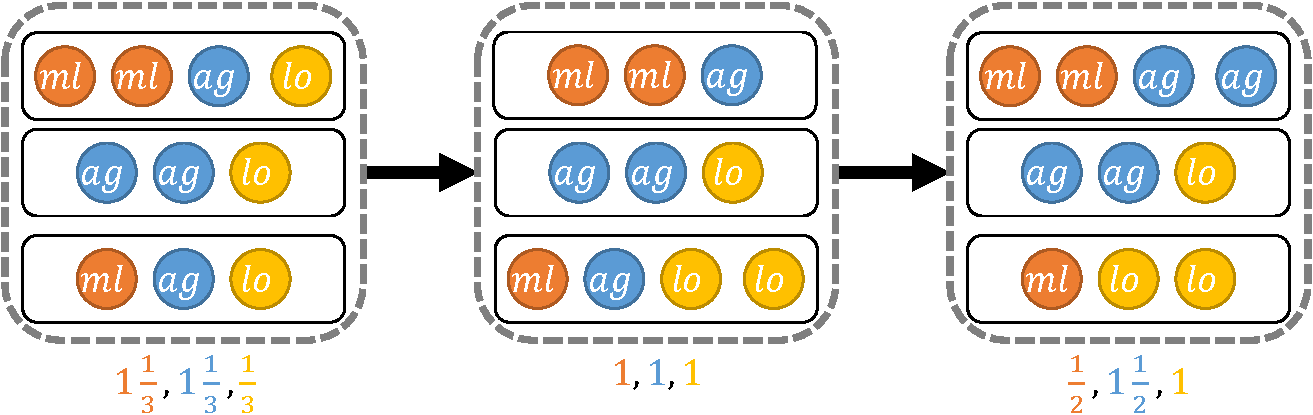
\includegraphics[width=\columnwidth]{example.pdf}
	\caption{Example 1 --- The $lo$ agent (represented as a yellow circle) in the top unit moves to the bottom unit, winning it over. This makes it possible for the $ag$ agent in the bottom unit to move to the top. The number indicate each groups score}
	\label{fig:example}
\end{figure}

\begin{example}
	Consider a multi-unit technology company. Each unit is in charge of one product, and each product can be developed using one of the three available technologies: machine learning (ML), algorithmic game theory (AGT), and logic. There are 10 developers in the company and 3 units, and in every unit there must be either 3 or 4 developers. The developers want that as many products as possible will be developed using their favorite technology.
	In case of a tie in a unit, the product will be developed using hybrid technology (i.e., fractional districts). 
	
	3 developers in the company are machine learning enthusiasts ($ml$), 3 believe in algorithmic game theory ($ag$) and the other 4
	support logic ($lo$) (the full preferences order is not needed for this example). The initial company partition is $V^0_1 = \{ml,ml,ag,lo\} $ $V^0_2 = \{ag,ag,lo\} $ and $V^0_3 = \{ml,ag,lo\}$.
	In the initial state, the first product is developed using ML techniques, the second product is developed using AGT and third combines all three approaches. 
	As can be seen in Figure~\ref{fig:example}, in the initial state, only a developer from the first unit can move to other units, due to the size constraints, and indeed 
	the developer that supports "$lo$" wants to move to the third unit, as this move will result in the third product be developed using logic approaches. That is, $V^1_1 = \{ml,ml,ag\} $ $V^1_2 = \{ag,ag,lo\} $ and $V^1_3 = \{ml,ag,lo,lo\}$.
	Now, the developer that supports "$a$" wants to move to the first unit and cause the first product to partly be developed using algorithmic game theory approaches and $V^2_1 = \{ml,ml,ag,ag\} $, $V^2_2 = \{ag,ag,lo\} $ and $V^2_3 = \{ml,lo,lo\}$.
	Assuming that the machine learning developers from $V^2_1$ prefer $lo\succ ag$, then no developer has an incentive to switch units and therefore the third state is stable. 
\end{example}



\section{Convergence}

The first step in our analysis is to try and see if there are cases in which the iterative process will converge.
\begin{table}[htp]
\caption{Summary of the cases our theorems prove for $b^{+}-b_{-}=1$. For $b^{+}-b_{-}>1$, see Theorem~\ref{nonConv}~(1), (2).}
\begin{center}
\begin{tabular}{|c |c c|}
\hline
& {\bf globalist} & {\bf lexicographic}\\
& {\bf utility}& {\bf utility}\\
\hline
{\bf fractional} &Theorem~\ref{nonConv}~(\ref{globFrac}) &Theorem~\ref{lexiFracConverge}\\
{\bf tie-breaking} &\emph{no convergence} &\emph{converges}\\
\hline
{\bf deterministic} &Theorem \ref{globalConverge} & Theorem \ref{lexiDetermConverge}\\
{\bf tie-breaking} &\emph{converges} &\emph{converges}\\
\hline
\end{tabular}
\end{center}
\end{table}


\begin{theorem}\label{globalConverge}
	If $b^{+}-b_{-}=1$ and agents are globalists and not vote-strategic and districts are not fractional, the iterative process will always converge to a Nash equilibrium, in which no agent wishes to change.
\end{theorem}
\begin{proof}
	First, we will show that under the theorem's conditions, the score of each district's winner is weakly monotonically increasing with the iterative process. If a district's size is $b_{-}$, no agent can leave, and if a new agent arrives, it will do so to change the winner outcome, and hence the new winner's score will be the same as the previous one (since all of its voters are still there), or strictly more. If the district size is $b_{+}$, at each point, the last transfer of a voter to the district (which made its size $b_{+}$) was needed to make this candidate win (otherwise the voter would not have moved). This means no supporters of the current winner can leave the district, therefore the score of the winner of the district will never decrease.
	
	Assume for contradiction that the process does not converge and results in a cycle. Since each district's maximal score is weakly monotonically increasing, districts' maximal scores during the cycle always stay the same. Of all the voters that move let $C'$ be the set of candidates they vote for, and let $c'\in C'$ be the candidate of that set that is highest ranked in the tie-breaking rule. Let $v$ be a voter that votes for $c'$. Once $v$ moves to a new district and $c'$ wins there, there is no way for any other candidate to dislodge $c'$. So $v$ has no reason to ever continue moving in the cycle, contradicting its existence.
\end{proof}



\begin{theorem}\label{lexiDetermConverge}
	If $b^{+}-b_{-}= 1$ with lexicographic, not vote-strategic voters and districts are not fractional the iterative process will always converge to a Nash equilibrium, in which no agent wishes to change.
\end{theorem}
\begin{proof}
	Assume for contradiction that there are cycles and let $\mathcal{S}=S^{1}\rightarrow S^{2}\rightarrow\cdots\rightarrow S^{l}\rightarrow S^{1}$
	be a cycle, where each $S \in \mathcal{S}$ is a state that holds all the relevant information. 
	
	First, observe that in every district one voter leaves, one voter
	joins and so on, because $b^{+}-b_{-}=1$. Further,
	voters would join districts only if they could influence the result
	in their new districts. For every state $S\in\mathcal{S}$, district $D \in \mathcal{D}$ and candidate
	$c \in C$ let $s\left(c,D,S\right)$ be the number of votes in district
	$D$ at state $S$ for candidate $c$. Let $w(D,S) \in C$ be the winner in district $D$ at state $S$.
	
	Let $C'\subset C$ be the set of candidates that become victorious
	during the cycle $\mathcal{S}$, and let $z\in C'$ be the lowest
	candidate in $C'$ according to the tie breaking rule. Let $D \in \mathcal{D}$
	be a district in which $z$ becomes victorious during $\mathcal{S}$
	and let $\left(v_{1},\dots, v_{\ell_{D}},v_{1}\right)$ be the ordered
	set of voters that joined district $D$ during $\mathcal{S}$ and
	let $\left(r_{1},\dots, r_{\ell_{D}},r_{1}\right)$ be the ordered set
	voters that left district $D$ during $\mathcal{S}$. Assume without
	loss of generality, that first voter $v_{1}$ joined district $D$
	and then voter $r_{1}$ left district $D$. Further, assume without
	loss of generality that voter $v_{1}$ supports candidate $z$.
	Consider the move $S^{1}\overset{v_{1}\rightarrow D}{\rightarrow}S^{2}\in\mathcal{S}$
	when voter $v_1$ joined district $D$.
	
	Now, there are two possible cases:
	\begin{description}
		\item [Case I: Voter $r_{1}$ does not support candidate $z$] Since candidate
		$z$ is the lowest ranked candidate, according to the tie breaking
		rule, who became victorious in district $D$ during the cycle $\mathcal{S}$,
		it must hold that $s\left(z,D,S^{2}\right)\geq s\left(c,D,S^{2}\right)+1$,\footnote{$s(x,y,z)$ denotes score of candidate $x$ in district $y$ for state $z$.} for every other candidate $c\in C$, $c\neq z$. As voter $r_{1}$ does not
		support candidate $z$, before $v_{2}$ joined district $D$, the
		winner was candidate $z$, and therefore after $v_{2}$ joined district
		$D$ in state $S^{h}$ there were exactly two candidates (including $z$) with $s\left(\cdot,D,S^{h}\right)\geq s\left(z,D,S^{2}\right)$.
		Because voters alternately join and leave district $D$ and voters
		would join a district only if they could influence the result,
		it holds that in every $S\in\mathcal{S}$ there is a candidate
		with 
		$
		s\left(\cdot,D,S\right)\geq s\left(z,D,S^{2}\right)\label{eq:eq1-1-1-2}
		$.
		However, if in state $S^{1}$ there was a candidate with $s\left(c,D,S^{1}\right)\geq s\left(z,D,S^{2}\right)$
		then voter $v_{1}$ could not make candidate $z$ victorious.
		
		\item[Case II: Voter $r_{1}$ does support candidate $z$] When $r_{1}$ left
		district $D$ they joined district $D'$. If the next voter to
		leave district $D'$ does not support candidate $z$ then we are back at Case I. Therefore, there is a cycle of $z$'s supporters
		that join and leave districts. Consider voter $v$ that left district
		$D$ and join district $D'$ in the move $S\overset{D \rightarrow v\rightarrow D'}{\rightarrow}S'$.
		As the last voter to join district $D$ also supports candidate $z$
		it must hold that $w\left(D,S\right)=z$, $w(D',S)\neq z$, $w(D,S')\neq z$
		and $w(D',S')=z$.\footnote{$w(x,y)$ denotes the winner in district $x$ in state $y$.} Let $w(D',S)=c$ and $w(D,S')=c'$, because $v$
		moved from $D$ to $D'$ it must hold $c\precneqq_{v}c'$, i.e., voter $v$ prefers candidate $c'$ over candidate $c$. Consider
		the directed graph $G_{v}=(C,E_{v})$ where the nodes are the candidates
		and there is a directed edge $\left(c,c'\right)\in E_{v}$ if and
		only if there is a move $S\overset{D \rightarrow v\rightarrow D'}{\rightarrow}S'\in\mathcal{S}$
		such that $w(D',S)=c$ and $w(D,S')=c'$. Because $\mathcal{S}$ is
		a cycle, after $v$ joins a district they leave the district and
		therefore the in-degree of a node $c\in G_{v}$ equals to its out-degree,
		and thus there is a cycle in $G_{v}$. However, for every directed
		edge $\left(c,c'\right)\in E_{v}$ it holds that $c \precneqq_{v}c'$, reaching a 
		contradiction.\end{description}\end{proof}

\begin{figure}
	\centering
	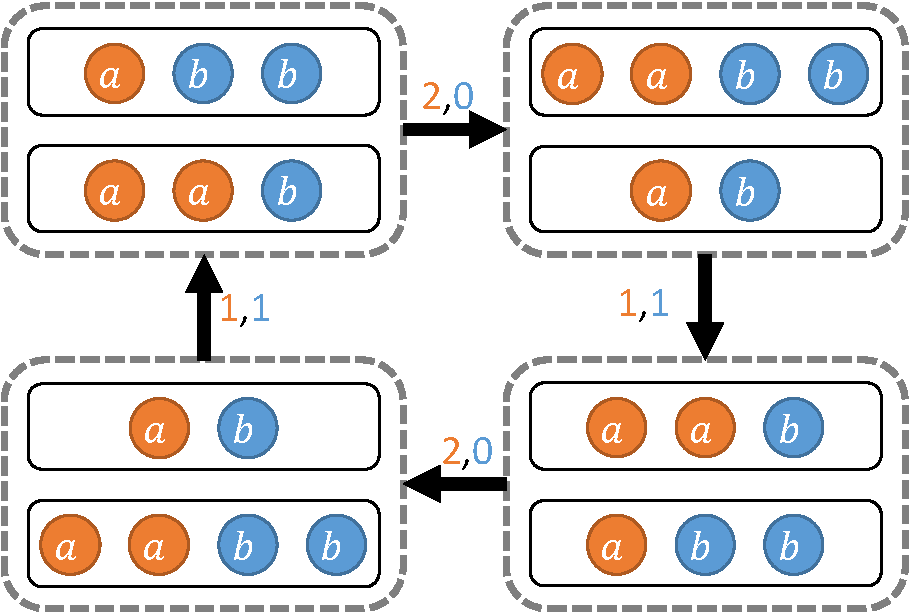
\includegraphics[width=0.7\columnwidth]{cycle_1.pdf}
	\caption{A cycle occurs, assuming districts are deterministic tie-breaking in each district is in $a$'s favor, and either agents are lexicographic, or the global tie-breaking is for $b$. On each edge is the score vector induced by this move.}
	\label{fig:cycle1}
\end{figure}
\begin{theorem}\label{lexiFracConverge}
	If $b^{+}-b_{-}=1$ with fractional districts and lexicographic, not vote-strategic voters, the iterative process will always converge to a Nash equilibrium, in which no agent wishes to change.\end{theorem}
\begin{proof}
	
	Again, assume for contradiction that there are cycles and let $\mathcal{S}=S^{1}\rightarrow S^{2}\rightarrow\cdots\rightarrow S^{l}\rightarrow S^{1}$
	be a cycle.
	
	As before, note that in every district one voter leaves, one voter
	joins and so on; and
	voters would join districts only if they could influence the result
	in their new districts.
	
	Now there are three possible cases:
	\begin{description}
		\item[Case I:] This is the case if during the cycle at some state $S\in\mathcal{S}$ for some $D \in \mathcal{D}$:
		$\left|\arg\max_{c \in C}s\left(c,D,S\right)\right|=1$. Let $c^{*}\in C$, $D \in \mathcal{D}$, $S^{1}\overset{v\rightarrow D}{\rightarrow}S^{2}\in\mathcal{S}$
		such that $\arg\max_{c \in C}s\left(c,D,S^{2}\right)=\left\{ c^{*}\right\} $ and in this case I, the next voter to leave district $D$ does not support candidate $c^{*}$.
		Let voter $v\in V$ be the voter that joined $D$ in the move
		$S^{1}\overset{v\rightarrow D}{\rightarrow}S^{2}$, let voter $v'\in V$
		be the next voter to join $D$ in the move $S^{h}\overset{v'\rightarrow D}{\rightarrow}S^{h+1}\in\mathcal{S}$,
		and let voter $u$ be the voter that left $D$ after $v$ has joined
		and before $v'$ has joined. As voters only join districts if they
		can influence the results, and voter $u$ did not support candidate
		$c^{*}$ it holds that there are two candidates in state $S^{h+1}$
		with $s\left(\cdot,D,S^{h+1}\right)=s\left(c^{*},D,S^{2}\right)$,
		and therefore for every $S\in\mathcal{S}$ there exists a candidate
		with $s\left(\cdot,D,S\right)=s\left(c^{*},D,S^{2}\right)$. It is
		a contradiction to the fact that before $v$ joined district $D$,
		$\max_{c \in C}s\left(c,D,S^{1}\right)=s\left(c^{*},D,S^{2}\right)-1$.
		
		\item[Case II:] This is the case if during the cycle at some state $S\in\mathcal{S}$ for some $D \in \mathcal{D}$:
		$\left|\arg\max_{c \in C}s\left(c,D,S\right)\right|=1$, however (unlike case I), this is the case if at
		any point that $\arg\max_{c \in C}s\left(c,D,S\right)=\left\{ c^{*}\right\} $
		for $c^{*}\in C$, $D \in \mathcal{D}$, $S\in\mathcal{S}$ the next voter
		to leave district $D$ supports candidate $c^{*}$. In that case, let $c^{*}\in C$,
		$D \in \mathcal{D}$, $S^{1}\overset{v\rightarrow D}{\rightarrow}S^{2}\in\mathcal{S}$
		such that $\arg\max_{c \in C}s\left(c,D,S^{2}\right)=\left\{ c^{*}\right\} $
		and let $u\in V$ be the next voter to leave district $D$ and joined
		district $D'$ in the move $S^{h}\overset{D \rightarrow u\rightarrow D'}{\rightarrow}S^{h+1}\in\mathcal{S}$.
		As voter $u$ supports candidate $c^{*}$, and $\arg\max_{c \in C}s\left(c,D,S^{h}\right)=\left\{ c^{*}\right\} $
		it must hold that $\arg\max_{c \in C}s\left(c,D',S^{h+1}\right)=\left\{ c^{*}\right\} $
		and the next voter to leave district $D'$ also supports candidate
		$c^{*}$. Hence, there is a cycle of $c^{*}$'s supporters that leave
		join and districts. Similarly to the proof of Theorem~\ref{lexiDetermConverge} (case II),
		because voters leave their district only if they strictly prefer the
		new outcome, this dynamic cannot cycle.
		
		\item[Case III:] This is the case if during the cycle $\mathcal{S}$, for every $S\in\mathcal{S}$, $D \in \mathcal{D}$:
		$\left|\arg\max_{c \in C}s\left(c,D,S\right)\right|>1$. In that case,
		when a voter $v\in V$ that supports candidate $c^{*}$ leaves district
		$D$ and joins district $D'$ in the move $S^{1}\overset{D \rightarrow v\rightarrow D'}{\rightarrow}S^{2}\in\mathcal{S}$
		it must hold that $c^{*}\in\arg\max_{c \in C}s\left(c,D,S^{1}\right)$
		and $c^{*}\in\arg\max_{c \in C}s\left(c,D',S^{2}\right)$ and in addition, due to the fractional character of districts,
		\begin{equation}
		\left|\arg\max_{c \in C}s\left(c,D',S^{2}\right)\right|<\left|\arg\max_{c \in C}s\left(c,D,S^{1}\right)\right|\label{eq:th2_eq_1}
		\end{equation}
		also note that 
		\begin{equation}
		\left|\arg\max_{c \in C}s\left(c,D,S^{1}\right)\right|=\left|\arg\max_{c \in C}s\left(c,D,S^{2}\right)\right|+1\label{eq:eq:th2_eq_2}
		\end{equation}
		and 
		\begin{equation}
		\left|\arg\max_{c \in C}s\left(c,D',S^{1}\right)\right|=\left|\arg\max_{c \in C}s\left(c,D',S^{2}\right)\right|-1.\label{eq:eq:th2_eq_3}
		\end{equation}
		Consider the following potential function\footnote{Definition of which can be found in \cite{MSZ13}.} 
		\begin{equation}
		\phi\left(S\right)=\sum_{D \in \mathcal{D}}\left|\arg\max_{c \in C}s\left(c,D,S\right)\right|^{2}\label{eq:eq:th2_eq_4}
		\end{equation}
		due to Equations \ref{eq:th2_eq_1}, \ref{eq:eq:th2_eq_2}, \ref{eq:eq:th2_eq_3} and \ref{eq:eq:th2_eq_4}
		it holds that $\phi\left(S^{1}\right)>\phi\left(S^{2}\right)$, which
		cannot happen in a cycle, as games with potential functions are guaranteed to converge to a Nash equilibrium~\cite{MS96}.\end{description}\end{proof}
	
	
\begin{figure}
	\centering
	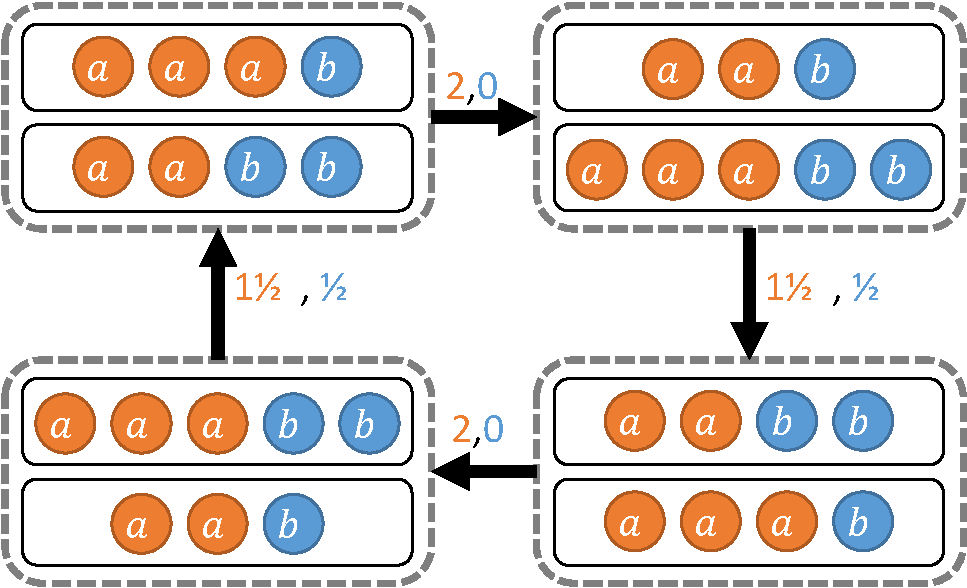
\includegraphics[width=0.75\columnwidth]{cycle_2.pdf}
	\caption{A cycle occurs, assuming districts are fractional and agents are lexicographic. On each edge is the score vector for the candidates induced by this move.}
	\label{fig:cycle2}
\end{figure}




These convergence proofs are tight, in the sense that almost any deviation from them, results in a setting that does not converge.

\begin{theorem}\label{nonConv}
	The following cases are not guaranteed to converge, and contain cases with cycles:
	\begin{enumerate}
		\item If $b^{+}-b_{-}\geq 2$ when districts are deterministic (not fractional) and agents are vote-strategic or not. {\bf [bounds of Theorem~\ref{globalConverge} and Theorem~\ref{lexiDetermConverge}]}
		\item If $b^{+}-b_{-}\geq 2$ when districts are fractional, and agents are lexicographic and either vote-strategic or not. {\bf [bound of Theorem~\ref{lexiFracConverge}]}
		\item If $b^{+}-b_{-}=1$ when districts are fractional and voters are globalist. {\bf [bound of Theorem~\ref{globalConverge}]}\label{globFrac}
	\end{enumerate}
	
\end{theorem}
\begin{proof}
	For item 1, when districts are deterministic, Figure~\ref{fig:cycle1} shows a cycle when tie-breaking $t$ in each district is $a\succ b$, and overall, $\tilde{t}$ is $b\succ a$.

	
	For item 2, when districts are fractional, Figure~\ref{fig:cycle2} shows a cycle, when agents are lexicographic.

	
	\begin{figure}
		\centering
		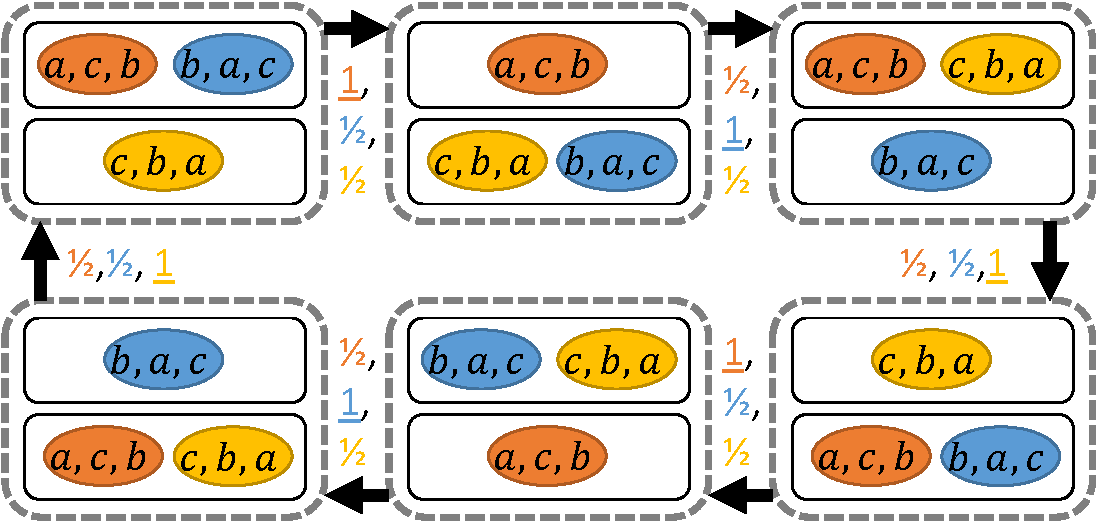
\includegraphics[width=0.9\columnwidth]{cycle_3.pdf}
		\caption{A cycle occurs, assuming districts are fractional and agents are globalist. On each edge is the score vector for the candidates induced by this move.}
		\label{fig:cycle3}
	\end{figure}
	For item 3, when districts are fractional and voters globalist, Figure~\ref{fig:cycle3} shows a cycle.
\end{proof}

\section{Simulations}

While the results on convergence are tight, we are interested to see the effects of the decentralized iterative dynamic on the overall welfare of the system. Moreover, as we have multiple parameters of the type of districts and types of agents, we are interested in exploring how (and if) are these parameters affect the efficiency of the process and how this affects the overall social welfare.

While the examples above demonstrated a relatively small number of candidates, when trying to simulate more of them, the question arises of determining the preference order of the voters. We have chosen to run each simulation both with randomized preferences as well as with single-peaked preferences. Single-peaked preferences are relevant when there is an agreed upon ordering of candidates on some axis (e.g., political right to left; location of public parks along a street; etc.). Every voter has a particular location on the axis which is its most favored location, and the farther away an option is from that location, the lower it is in the voter's preference order. Unlike randomized preferences, which can create quite unrealistic preference orders, there is a case to be made regarding these preferences (see \cite{Spr91}) and resembling realistic preferences (as \cite{End1715} note, elections are rarely purely single peaked, but they are closer than purely random models, as \cite{Ked09} indicates).

In order to calculate social welfare, in each simulation, we measure the percentage of voter that prefer the final state over the initial state.\footnote{
	In a case where a cycle occurred, we averaged over all the states of the cycle.} 

In order to simplify data analysis and comparison, we ran a few experiments with a large variety of voter numbers, but here we will present the extensive simulations we have done of the iterative dynamic with 53 voters (the number was useful due to the district size). We examined the effects of the number of districts (we ran simulations with 2,3,5 and 10), and the size of the gap between maximal and minimal group size -- $b^{+}-b_{-}$ (we ran simulations with 1,2,3,4,5).

A simulation setting included a choice of number of the district, a choice of the number of candidates, a choice of the size of gap, whether voter preferences were uniformly randomly generated or single-peaked, whether districts were fractional or deterministic, whether agents' utilities were global or lexicographic, and whether agents were vote-strategic or not. For each of these 320 potential settings, we ran 1,000 scenarios, each beginning in the truthful state (for vote-strategic agents), and advancing from there.
\begin{figure}
	\centering
	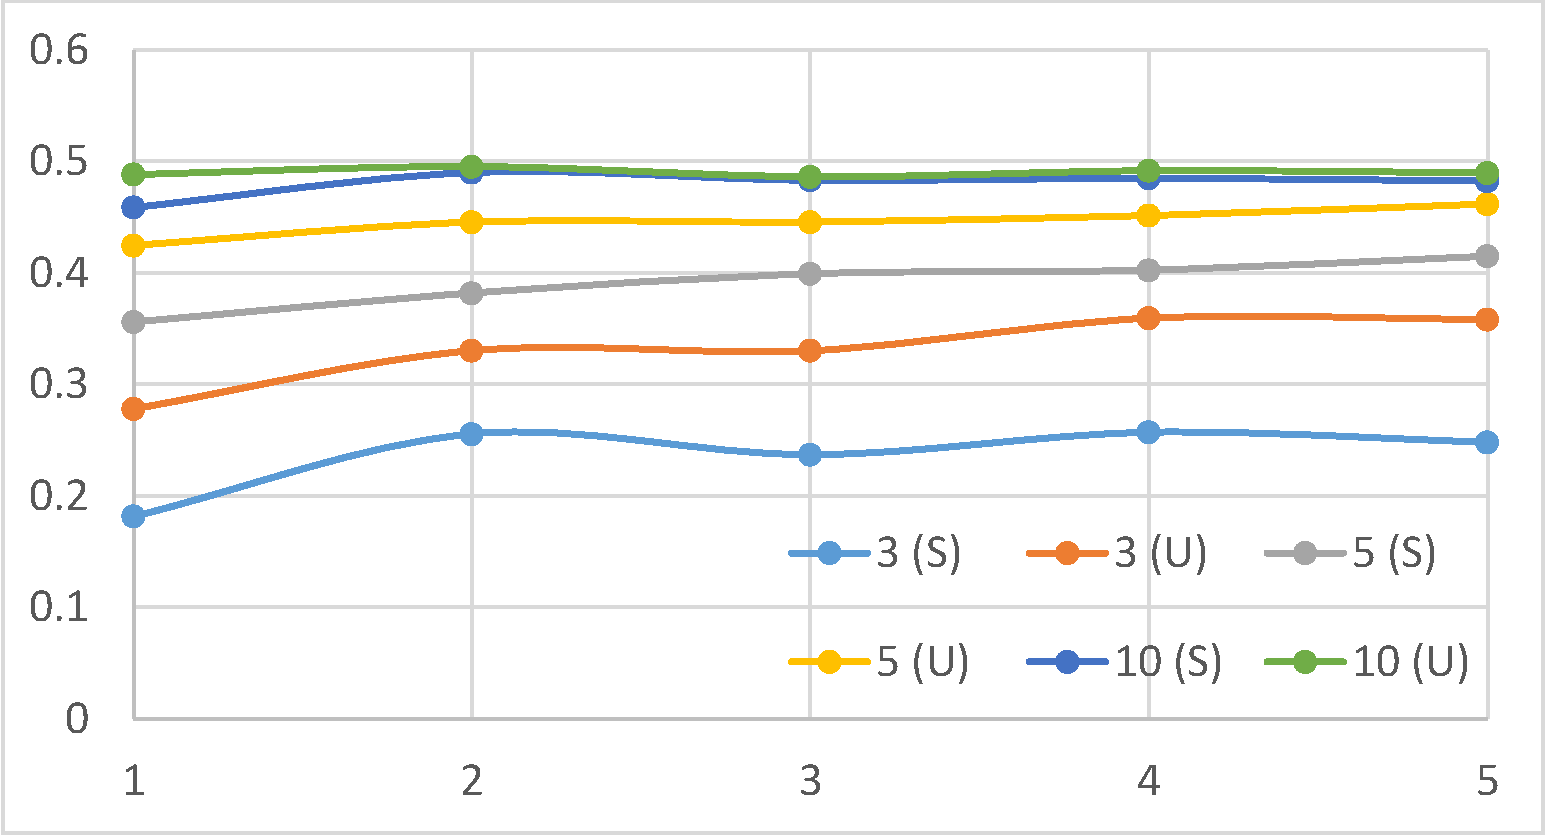
\includegraphics[width=0.9\columnwidth]{by_team__by_sp_rev_stats_agent_util_imp_v_53_tb_True_st_True_gr_False_can_8_N_1000_new.pdf}
	\caption{The average proportion of agents that prefer the final position over the opening position 
		for non-strategic agents with deterministic tie-breaking, lexicographic utility, according to the gap constraint (the $x$-axis) and number of districts for elections with 8 candidates.
		(S) marks single-peaked preferences vs. uniformly random ones (U)
	 Generally, as the gap constraints are loosened, agents can increase their welfare.}
	\label{fig:bytbrevlastnormnocyclev53stTruegrTruespTrueN10000}
\end{figure}


\section{Results}

Despite the theoretical convergence results, the most striking of the simulation results was that the rate of non-convergence was so small. It was, overall, slightly less than 0.66\%. While no setting had a particularly large amount of cycles, the number of districts did slightly increase them, as did using lexicographical utilities and using fractional districts. On average, 57\% of initial states were already in equilibrium, but this was highly volatile, and mostly appeared in settings with a small number of districts. 

Convergence happened in almost all cases within 13 steps. Single-peaked preferences took markedly less time (presumably, thanks to their more structured form), and global utility converged faster than lexicographic utility. 

The flexibility that is given to players to manipulate -- the maximal/minimal bounds over district sizes -- affects the outcome, though it was not necessarily monotonic. As can be seen in Figure~\ref{fig:bytbrevlastnormnocyclev53stTruegrTruespTrueN10000} (the $x$-axis is $b^+ - b_-$) the effect of the gap on all cases is almost identical
 -- even when the ``amplitude'' of the agents' social welfare is different (mostly dependent on district size and on distribution), the effect of changing the constraints is fairly consistent across all settings.
 This is also true when comparing the social welfare as a function of the number of district for fractional vs. deterministic tie-breaking.
As can be seen in Figure~\ref{fig:TieDiverge}, the utility increase as the number of districts grows (the $x$-axis), and generally speaking under fractional settings, the agents tend to prefer the final 
state more than under deterministic tie-breaking settings.



\begin{figure}
	\centering
	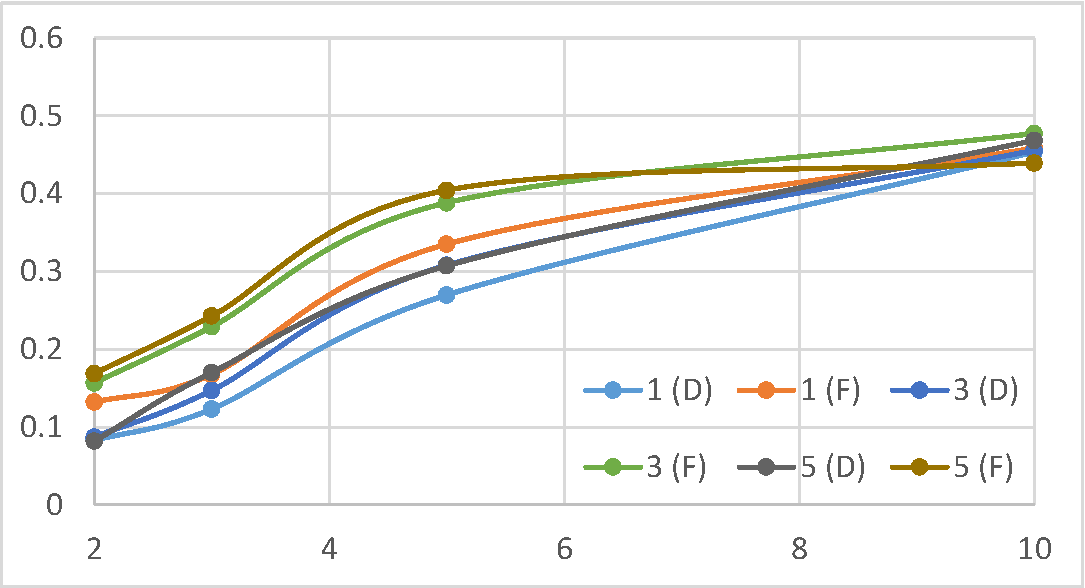
\includegraphics[width=\columnwidth]{by_gap_by_tb_rev_stats_agent_util_imp_v_53_st_False_gr_False_sp_True_can_5_N_1000_new.pdf}
	\caption{The average proportion of agents that prefer the final position over the opening position for non-strategic agents with lexicographic utility and 5 candidates, according to number of districts (the $x$ axis) and various gaps. (F) marks fractional tie-breaking vs. deterministic one (D).}
	\label{fig:TieDiverge}
\end{figure}



\begin{figure}
	\centering
	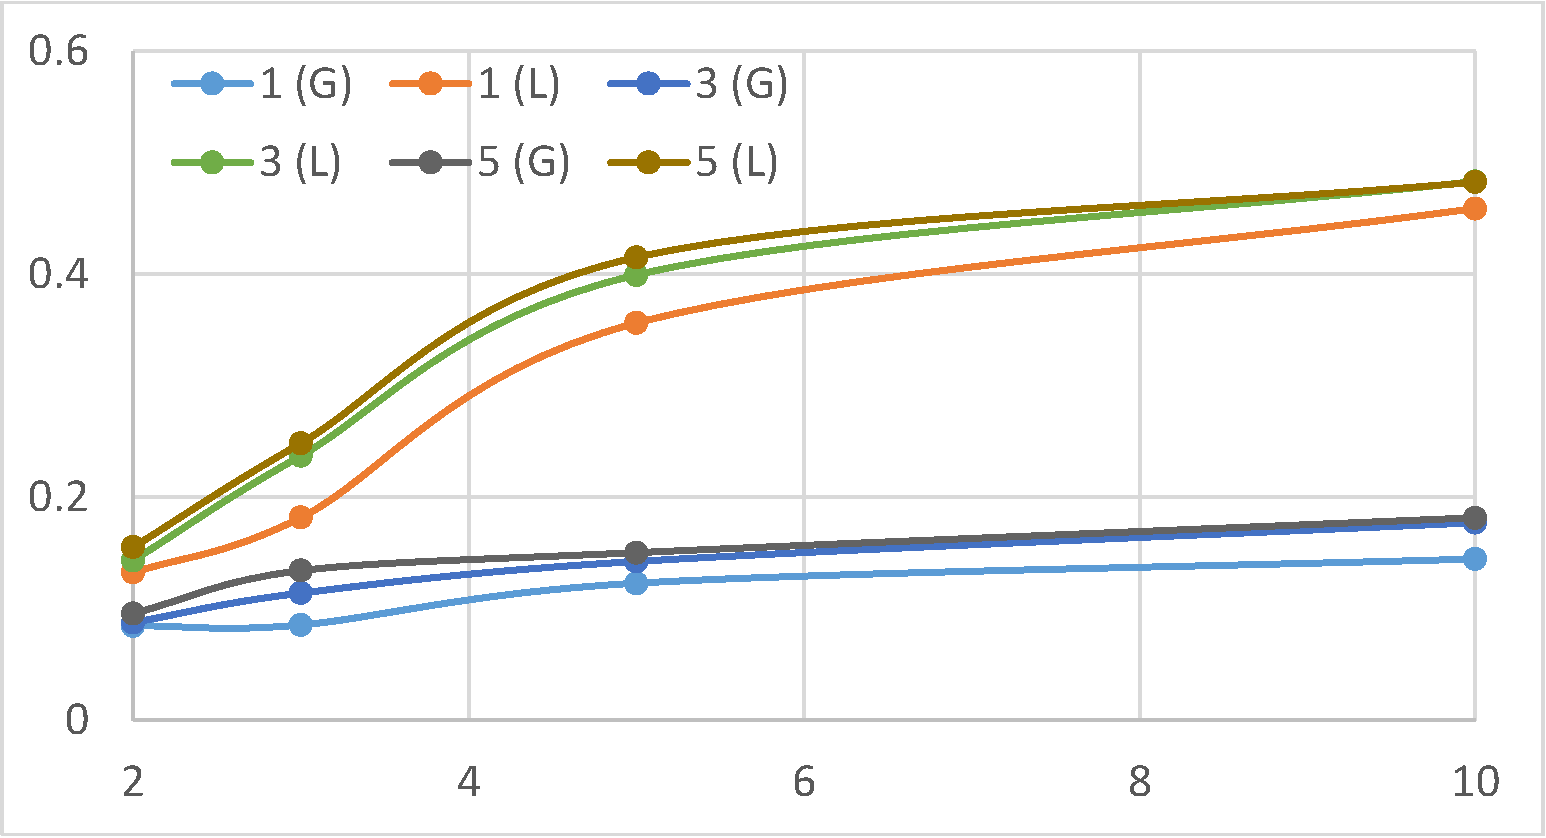
\includegraphics[width=\columnwidth]{by_gap_by_gr_rev_stats_agent_util_imp_v_53_tb_True_st_True_sp_True_can_8_N_1000_new.pdf}
	\caption{The average proportion of agents that prefer the final position over the opening position 
for strategic agents with deterministic tie-breaking and 8 candidates, according to number of districts (the $x$ axis) and various gaps. (L) marks lexicographic preferences vs. globalist ones (G).}
	\label{fig:LocalBest}
\end{figure}
The difference in utility between globalists and lexicographic agents is quite significant (almost $250\%$ more), as can be seen in Figure~\ref{fig:LocalBest}, an advantage that is consistent (though with different magnitudes) when changing number of candidates, tie-breaking system, and whether agents are strategic or not. This has to do with the greater ability of lexicographic agents to be partially satisfied -- several agents, with opposing views can be satisfied. However, the growth is quite dramatic. Furthermore, notice that smaller gaps produce less utility for the agents, while larger gaps presumably allow greater flexibility to the manipulating agents.



Beyond lexicographic agents' greater utility, global agents' distribution can effect their utility significantly. As can be seen in Figure~\ref{fig:SPGlob}, single-peaked agents were almost half the utility compared those whose preferences were allocated uniformly at random. Notice that, as before, in general, higher gap agents were more successful.

\begin{figure}
	\centering
	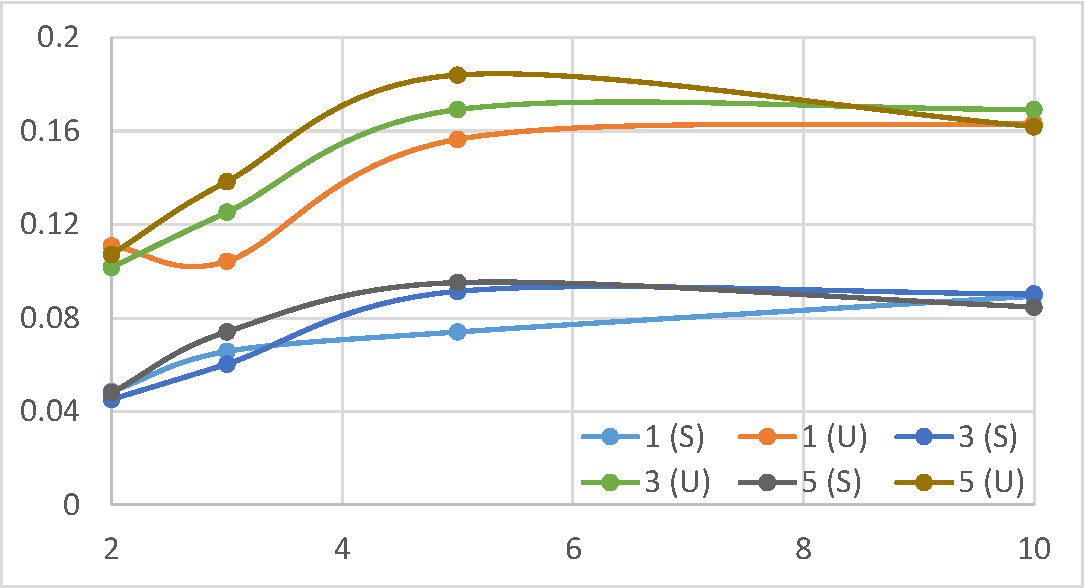
\includegraphics[width=\columnwidth]{by_gap_by_sp_rev_stats_agent_util_imp_v_53_tb_True_st_False_gr_True_can_5_N_1000_new.pdf}
	\caption{The average proportion of agents that prefer the final position over the opening position 
		 for non-strategic agents with deterministic tie-breaking, global utility and 5 candidates, according to number of districts (the $x$ axis) and various gaps. (S) marks single-peaked preferences vs. uniformly random ones (U).}
	\label{fig:SPGlob}
\end{figure}

We should note that one of the most surprising outcomes is that strategic agents did not, ultimately, have a meaningfully better utility than non-strategic agents. In a sense, all agents could save themselves the effort, and just not bother with strategizing.

\section{Discussion}

The ``reverse gerrymandering'' setting, presented in this paper, may sound slightly unnatural at first blush, since people do not usually get to jump between voting districts (though \cite{BM12} worked on such a setting). However, we believe that when viewed from the perspective of people participating in workplace committees, with their overlapping organizational influence, they do indeed strategize on where they could be more influential, and they move if they find a better position. In a more futuristic outlook, as autonomous systems become more common, the issue of these agents will need to be finding on their own where they are pivotal to help, and when will it be wrong to move.
We presented here both theorems on the properties of this dynamic, and also explored it empirically (including for cases which we showed could not converge, hence an empirical examination is the main tool for analysis), discovering some key issues on the effect of changing the agent preference model, and the effect of district size on the agent. There is still much to discover -- what other preference models work well with this setting; understanding better the effect of the gap constraints on social welfare; and combining various different types of agents in the same simulation, examining how their differences interact.

\section*{Acknowledgments}
This research has been partially supported by the HUJI Cyber Security Research Center in conjunction with the Israel National Cyber Directorate (INCD) in the Prime Minister's Office.
%References and End of Paper
%These lines must be placed at the end of your paper
\bibliography{general}
\bibliographystyle{aaai}
\end{document}
